\section{General Analysis}

% The hypothesis was that the algorithms should be able to finish training after 1000 episodes and that SARSA would perform better, but this was not the case.
% Looking at the provided graph, we aren't able to conclude if one algorithm is better than the other.
% We think that the reason the training didn't finish is that the number of episodes as well as the hyperparameters weren't optimal. 
% So in order to rectify this, we plan on increasing the number of total episodes. 
% In addition, we are planning to do sensitivity analysis with the hyperparameters and will compare SARSA and Q-Learning further.
% In particular, we think the performance might increase if the value of epsilon is higher that allows the agent to take more random actions and explore the action space more effectively.

\subsection{Hypothesis 1}

For hypothesis 1, we compared the performance of Q Learning and SARSA learning, over a static $\epsilon$ value of 0.5

Looking at the figures, we can see that [...]

\subsection{Hypothesis 2}

We explored three different methods of $\epsilon$ decay. First, $\epsilon$ is kept static at a value of 0.5. Second, 
$\epsilon$ followed the decaying function of $\epsilon = 0.5 * \frac{1}{no. of episodes}$. Finally,
$\epsilon$ follows the exponential decaying fucntion of $\epsilon = 0.5 * e^{-0.001*no. of episodes}$

For SARSA, comparing the three methods of $\epsilon$ decay, yields the following results:

\begin{figure}[H] %h forces the figure to be inserted right here
    \centering
    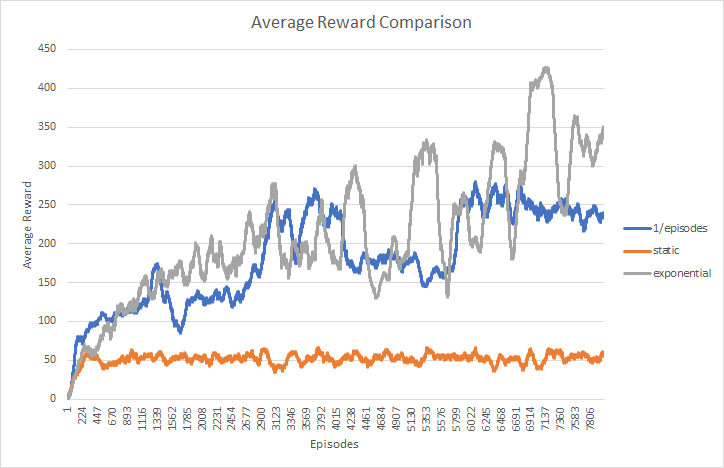
\includegraphics[width=1\linewidth]{epsilon-decay-comparison.png}
    \caption{Average Reward of SARSA, Comparing DIfferent $\epsilon$ Decay}
\end{figure}

Additionally, the mean and standard deviation for each method are as follows:

\begin{table}[H]
    \begin{tabular}{lll}
    \hline
    Method      & Mean   & Standard Deviation \\ \hline
    Static      & 52.07  & 7.545              \\
    1/Episodes  & 171.9  & 15.454             \\
    Exponential & 207.45 & 80.459             \\ \hline
    \end{tabular}
    \caption{Mean of Average Reward and Standard Deviation}
\end{table}

As these results show, for the SARSA algorithm, exponential decay of $\epsilon$ performed the best.

Next, for Q Learning, the comparison graph is as follows:
% SARSA with static epsilon = 0.5: mean: 52.07, standard deviation: 7.545
% SARSA with static epsilon = 0.0: mean: 130.09, standard deviation: 15.454
% SARSA with epsilon = 0.5*(1/episode): mean: 171.9, standard devidation: 30.504 (episode-related decay?)
% SARSA with epsilon = 0.5*e^(-0.001*episode): mean: 207.45, standard deviation: 80.459 (exponential decay)

% \section{Difficulties Encountered}

% One of the main difficulties we have with this project is figuring out a good way to discretize the state space of the environment.
% As such, this hindered our abilities to perform more experiments in a timely manner.
% Fortunately, we came across the \textbf{digitize()} function from the \textbf{numpy} package that does the job quite well.

% Another issue that we are facing, due to the random nature of picking an action, no two runs are the same. Therefore, conducting some sort of
% sensitivity analysis for our hyperparameters has proven to be difficult. We have tried to solve this by setting a seed number at the beginning
% of our script, but that does not seem to be an effective solution yet.

% Additionally, for both algorithms, the result is unstable. For some runs, the rewards converged to an average of 50-55 after 200 episodes, and remains stable. However, divergence is encountered
% as well. This can be seen in the graph of Khoi's SARSA run. Therefore, it was hard to see if the agent was trained well or not.